\chapter{Grundlagen}
\label{ch:Grundlagen}


UDP

Beim User Datagram Protocol handelt es sich um ein verbindungsloses und in jeglicher Hinsicht ungeschütztes Protokoll, das auf der Transportebene (Schicht 4 im OSI-Schichtenmodell) arbeitet. Es bestehen keinerlei Mechanismen, die das korrekte Übertragen von Paketen gewährleisten. Hierzu zählen:

\begin{description}
	\item[Sicherheit] Die Sicherheit, dass Pakete überhaupt ankommen
	\item[Reihenfolge] Die Reihenfolge, in der Pakete ankommen
	\item[FlowControl] Ein Überlaufschutz des Empfängerspeichers (FlowControl)
	\item[CongestionControl] Stauvermeidung in der Übertragungskette (CongestionControl)
	\item[Angriffe] Schutz gegen Paketmanipulation von dritten
\end{description}

\begin{figure}
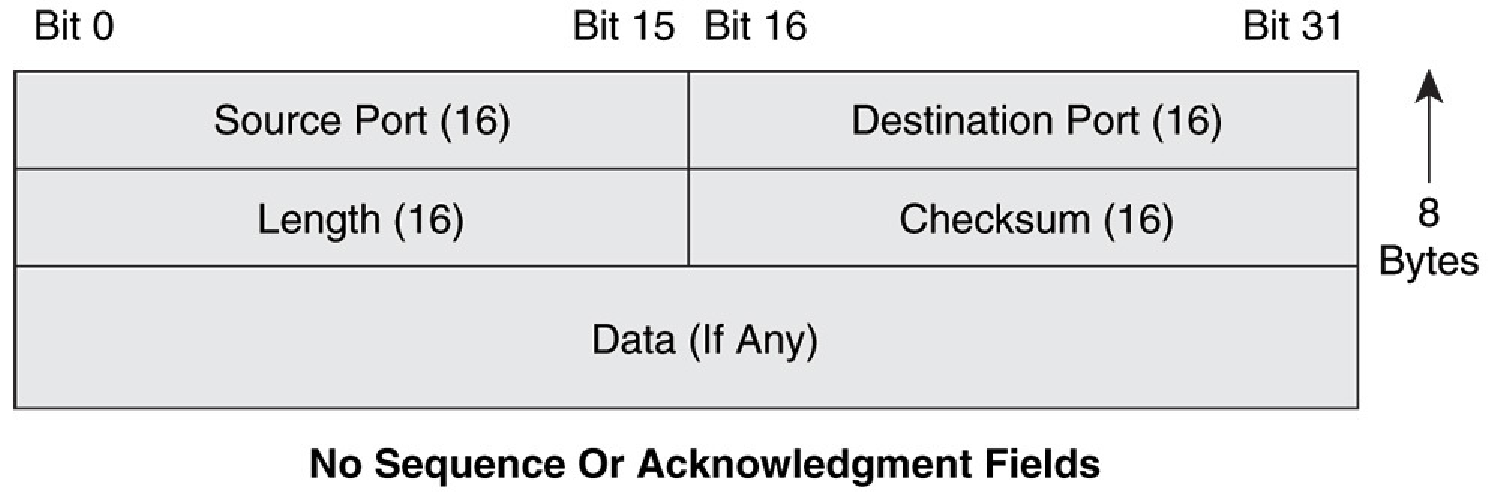
\includegraphics[width=\textwidth]{images/UDP_header.pdf}
\caption{UDP Header}
\label{fig:udp_header}
\end{figure}

Ein UDP Header besteht aus 8 Byte. Mit diesen 8 Byte werden lediglich Source-Port, Destination-Port, Länge und die Checksumme übertragen. Dieser vergleichsweise kleine Header (vgl. TCP mit etwa 20 Byte), führt zu einem geringen Overhead während der Übertragung, auch bei kleinen Paketen. Nachdem ein Paket gesendet wurde erfolgt keine Bestätigung des Pakets vom Empfänger. Durch diesen Uni-Direktionalen Sendevorgang entsteht wenig Traffic im Netzwerk. Falls gewisse Sicherheitsmechanismen gewünscht sind, müssen diese in höheren Schichten implementiert werden. \\
Aufgrund dieser Eigenschaften wird UDP in Bereichen eingesetzt, in denen es auf hohe Übertragungsgeschwindigkeit ankommt und eventuelle Paketverluste zu verkraften sind, bzw. von höheren Schichten aufgelöst werden.




\newpage


TCP

Beim Transmission Control Protocol handelt es sich um ein verbindungsorientiertes paketvermittelndes Protokoll. Mithilfe verschiedener Mechanismen wird sichergestellt, dass Pakete in der richtigen Reihenfolge ankommen, es zu keinen Staus kommt und dass Netzwerkknoten nicht überlaufen. Dadurch, dass das Protokoll verbindungsorientiert arbeitet, können beide Teilnehmer der Verbindung Daten ohne Anfragen senden. 

\begin{figure}
	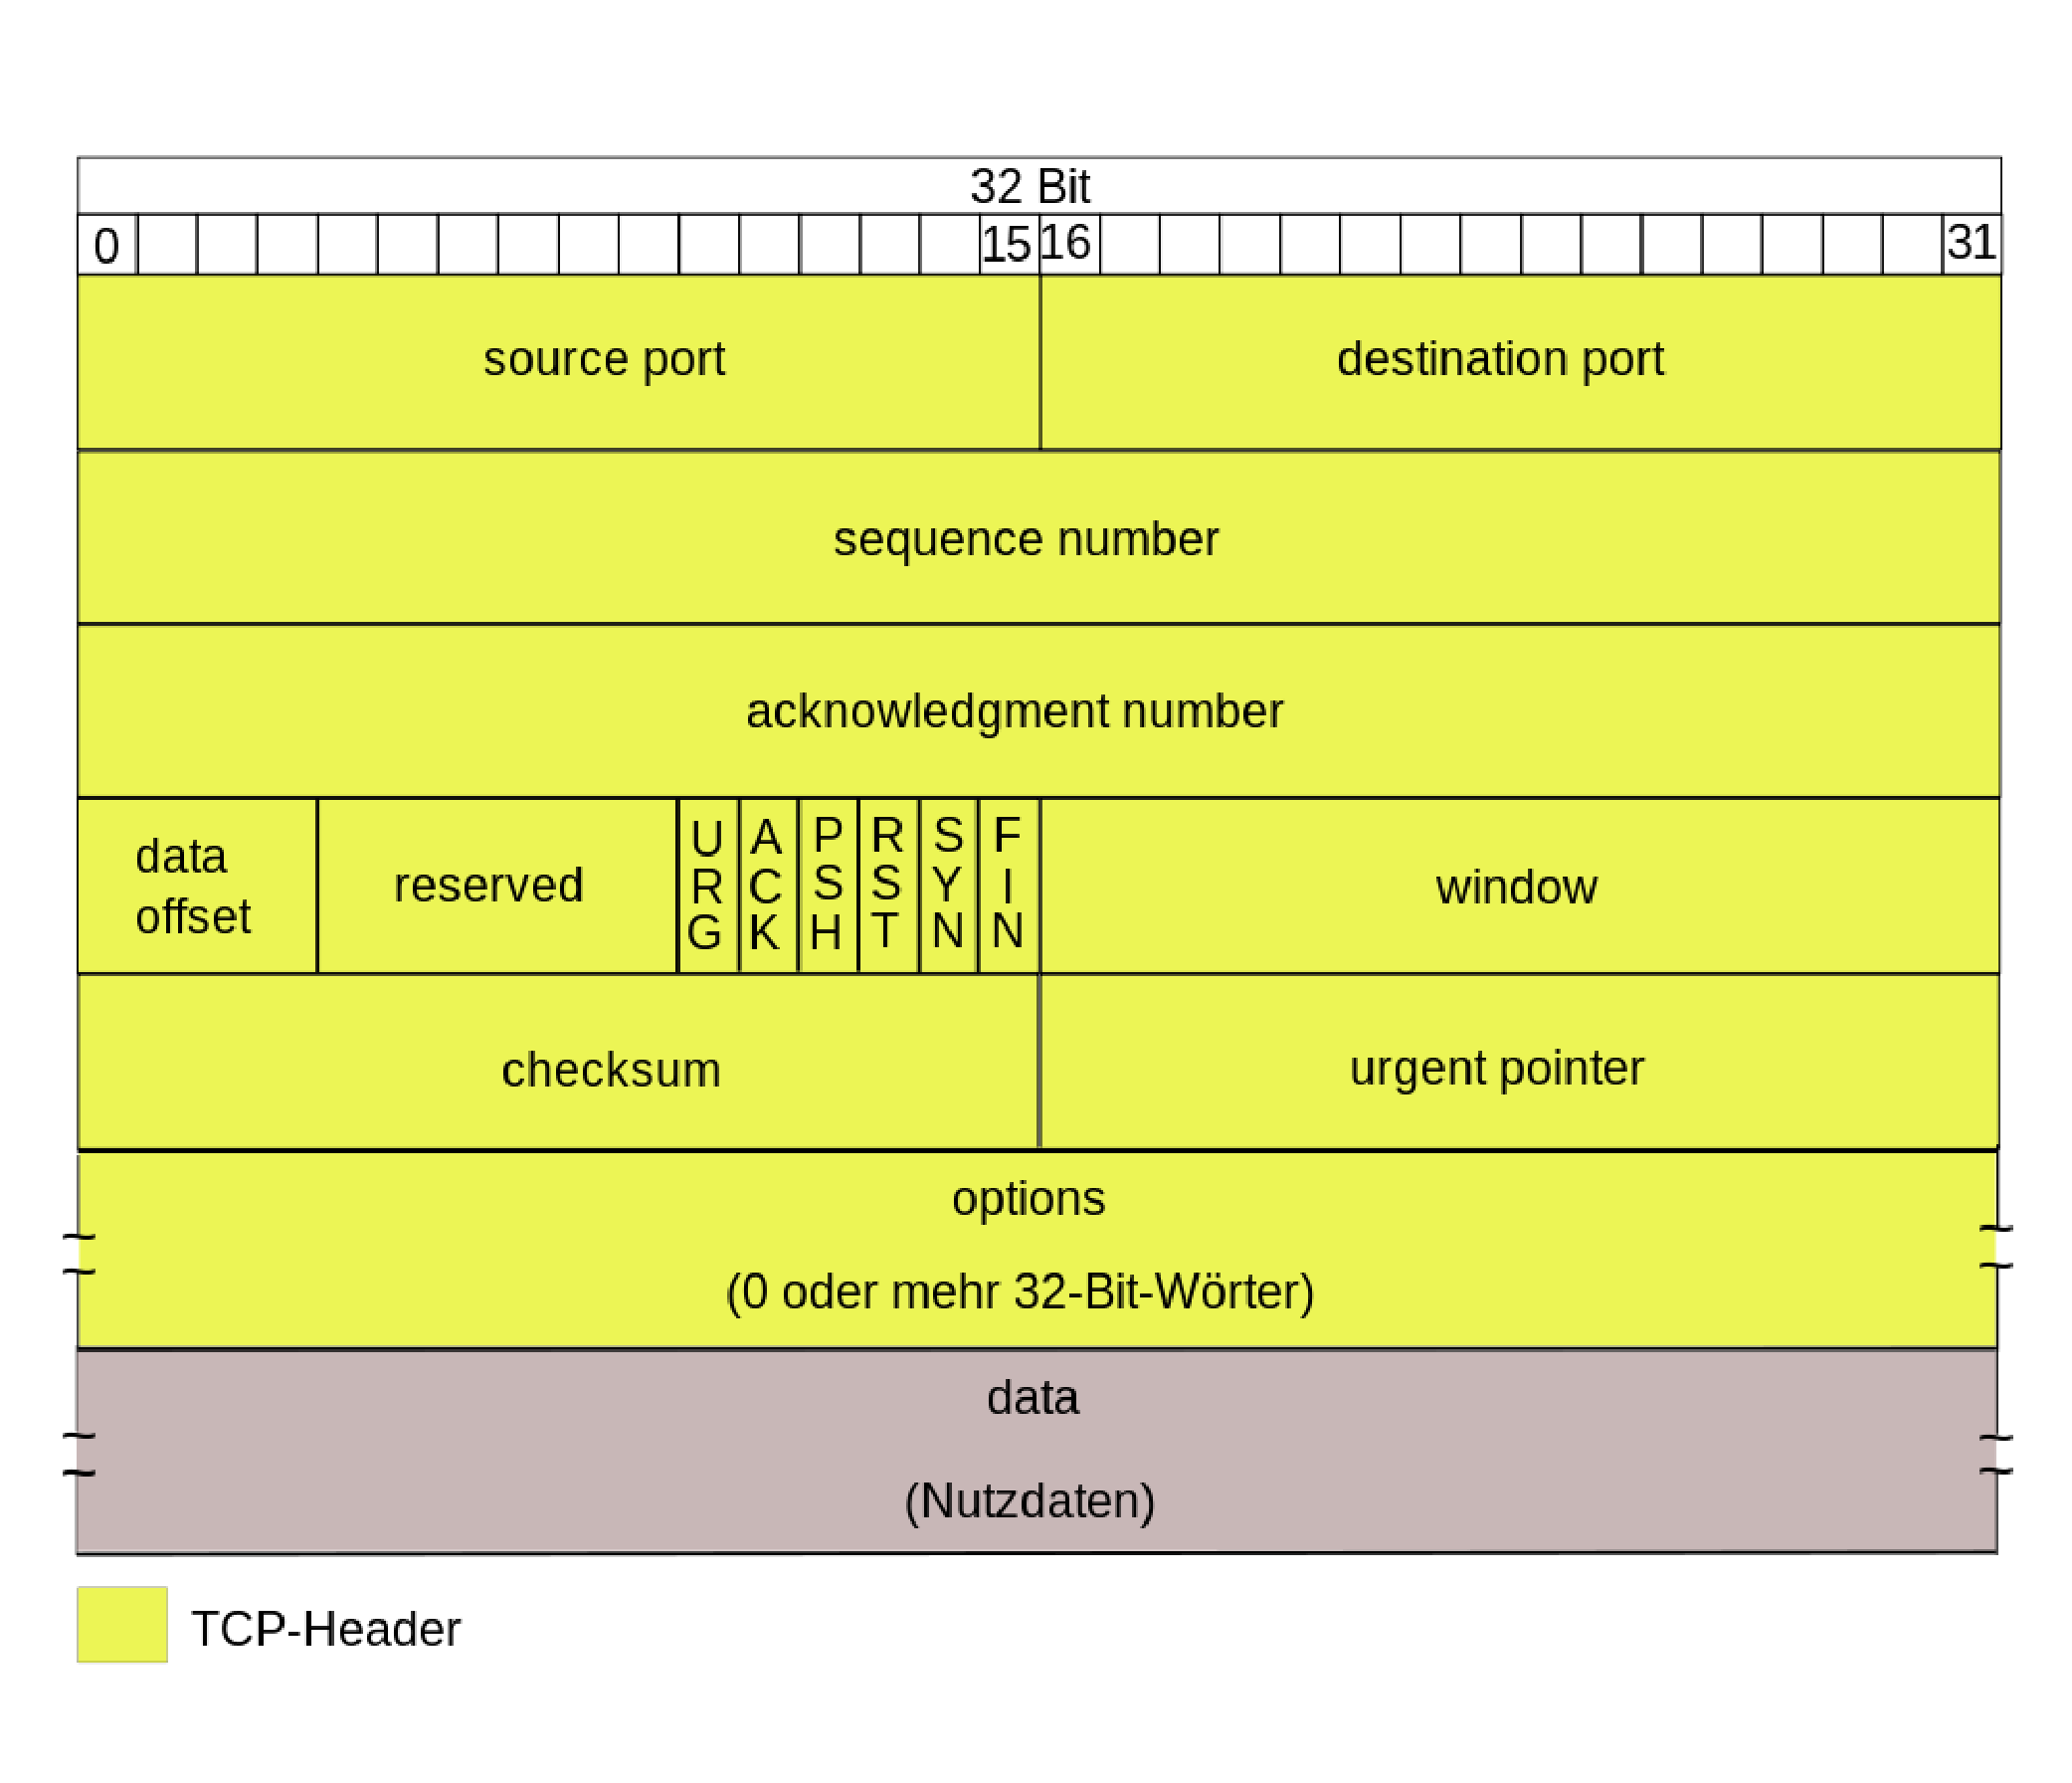
\includegraphics[width=\textwidth]{images/TCP_header.pdf}
	\caption{TCP Header}
	\label{fig:tcp_header}
\end{figure}

Durch den größeren Header und dem größeren Traffic, der das Protokoll verursacht, wird TCP für Anwendungen verwendet, bei denen ein Paketverlust ausgeschlossen werden soll, dafür aber eine etwas höhere Latenz in Kauf genommen werden kann. 
Die Verbindung wird über einen 3-Wege-Handshake hergestellt. Hierbei sendet ein Teilnehmer eine Anfrage (syn), diese wird bestätigt (syn ack) woraufhin die Bestätigung erneut bestätigt wird. In diesem dritten Schritt werden meist bereits die ersten Nutzdaten mitgesendet.
\begin{figure}
	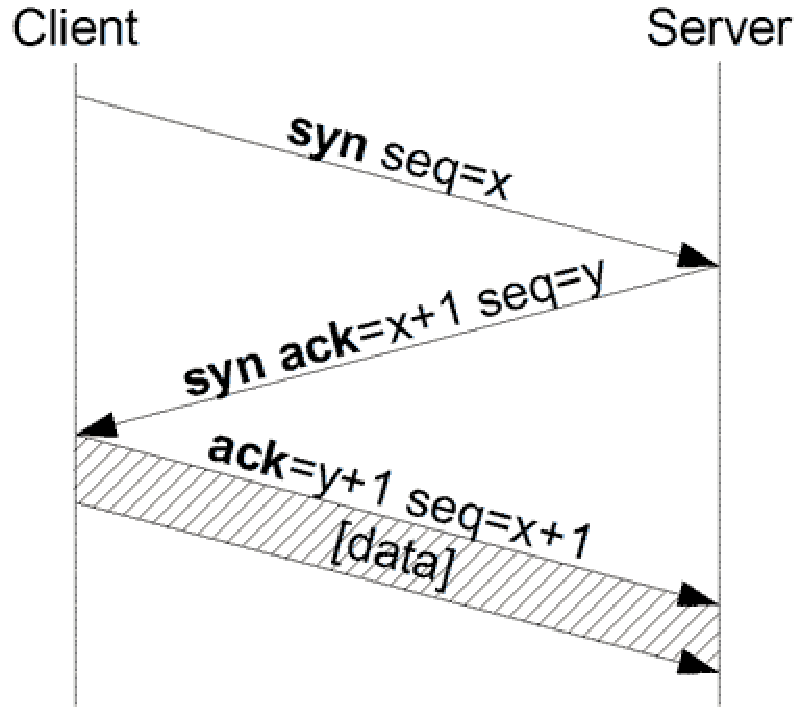
\includegraphics[width=\textwidth]{images/TCP_3wayhandshake.pdf}
	\caption{TCP 3-Wege-Handshake}
	\label{fig:tcp_3wayhandshake}
\end{figure}

Mithilfe von geordneten Sequenznummern und Acknowledgments werden alle empfangene Pakete bestätigt. Durch das Fehlen einer Sequenznummer erkennt der Empfänger den Verlust eines Pakets und teilt daraufhin dem Sender mit, dass es nicht angekommen ist. Für den Fall eines Verlusts des Acknowledgments, hat der Sender einen Timer, welcher nach einiger Zeit eine Retransmission des Pakets veranlasst, sofern kein Acknowledgment ankommen sollte.




HTTP

Das Hypertext Transfer Protocol ist ein zustandsloses Datenübertragungsprotokoll, das auf der Anwendungsschicht arbeitet. Am meisten wird das Protokoll für den Aufbau von Internetseiten verwendet, also von einem Webbrowser, jedoch ist das Aufgabenfeld nicht darauf beschränkt.

HTTP arbeitet mittels zwei Befehlsarten, dem Request und dem Response. Möchte ein Browser eine Datei von einem Server laden, so sendet er einen Request mit dem Namen der Datei. \\
Die möglichen Befehle sind: 
\begin{description}
	\item[GET] fordert eine Ressource auf dem Server an
	\item[POST] sendet Daten zur weiteren Verarbeitung zum Server
	\item[HEAD] fordert lediglich den HEADER eines Responses an, der auf einen GET-Request folgend würde
	\item[PUT] lädt eine Ressource auf den Server
	\item[DELETE] löscht eine Ressource auf dem Server (Wird kaum verwendet)
	\item[TRACE] sendet die Anfrage, so wie sie empfangen wurde zurück
	\item[OPTIONS] liefert eine Liste mit den vom Server unterstützten Optionen
	\item[CONNECT] wird für SSL-Tunneling verwendet
\end{description} Nachdem der Request beim Server eingegangen ist und verarbeitet wurde, sendet er einen Response. In diesem Response sind Informationen über Server und Datei enthalten, sowie die Nutzdaten, also die angefragte Datei. In Abbildung \ref{fig:http_request_response} ist eine solche Kommunikation dargestellt.
-- 
\begin{figure}
	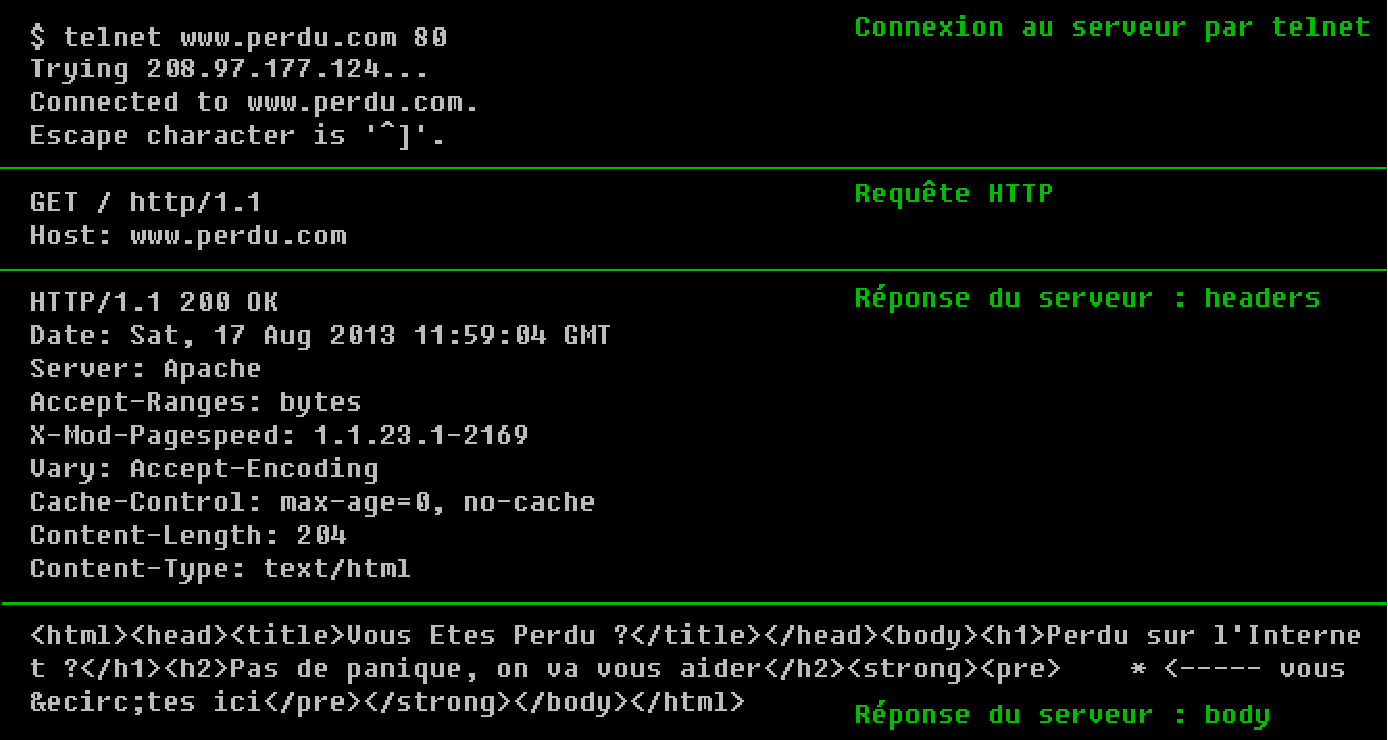
\includegraphics[width=\textwidth]{images/HTTP_request_response.pdf}
	\caption{HTTP Kommunikation}
	\label{fig:http_request_response}
\end{figure}



WebSockets

Das WebSocket-Protokoll ist ein Netzwerkprotokoll, das auf TCP und HTTP basiert. In diesem Protokoll ist es möglich, eine bidirektionale Verbindung zwischen einer Webanwendung und einem WebSocket-Server herzustellen. Im Gegensatz zu reinem HTTP ist es hierbei möglich, dass der Server ohne einen vorhergehenden Request des Clients, Daten an den Client sendet. Lediglich den Verbindungsaufbau muss der Client initiieren. Dies wird realisiert, indem die TCP-Verbindung nach dem Verbindungsaufbau nicht sofort geschlossen wird. 
Eine WebSocket URL wird über die beiden Schemata wss und ws definiert, was für verschlüsselte und unverschlüsselte Verbindungen steht.

Der Verbindungsaufbau funktioniert über einen Handshake, der wie in HTTP üblich über einen Request und anschließenden Response erreicht wird. Aufgrund der Tatsache, dass die HTTP-Header nur beim Verbindungsaufbau gesendet werden und dadurch der Traffic durch den HTTP-Header gering ist, wird das Protokoll hauptsächlich von Anwendungen verwendet, die regelmäßige Kommunikation zwischen Client und Server verlangen, wie zum Beispiel Online-Spiele.



Jetty Webserver

Jetty ist eine Java-Implementierung eines Webservers. Durch seine geringe Größe ist es leicht, ihn in andere Software zu integrieren. Außerdem unterstützt Jetty die Möglichkeit WebSockets aufzubauen.